%4
\subsection{Új elemek verembe helyezése (push)}
\begin{frame}
  \begin{columns}[c]
    \column{0.5\textwidth}
      \begin{exampleblock}{\textattachfile{verem2.cpp}{verem2.cpp}}
        \vspace{-.2cm}
        \small
        \lstinputlisting[style=cpp,linerange={4-16},numbers=left,firstnumber=4]{verem2.cpp}
        \vspace{-.2cm}
      \end{exampleblock}
    \column{0.45\textwidth}
      
\includegraphics[width=\textwidth]{verem/verem01.pdf}
  \end{columns}
\end{frame}

%5
\begin{frame}
  \begin{columns}[c]
    \column{0.5\textwidth}
      \begin{exampleblock}{\textattachfile{verem2.cpp}{verem2.cpp}}
        \vspace{-.2cm}
        \small
        \lstinputlisting[style=cpp,linerange={4-16},numbers=left,firstnumber=4]{verem2.cpp}
        \vspace{-.2cm}
      \end{exampleblock}
    \column{0.45\textwidth}
      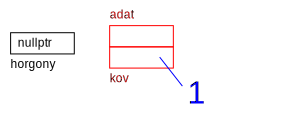
\includegraphics[width=\textwidth]{verem/verem02.pdf}
  \end{columns}
\end{frame}

%6
\begin{frame}
  \begin{columns}[c]
    \column{0.5\textwidth}
      \begin{exampleblock}{\textattachfile{verem2.cpp}{verem2.cpp}}
        \vspace{-.2cm}
        \small
        \lstinputlisting[style=cpp,linerange={4-16},numbers=left,firstnumber=4]{verem2.cpp}
        \vspace{-.2cm}
      \end{exampleblock}
    \column{0.45\textwidth}
      \includegraphics[width=\textwidth]{verem/verem03.pdf}
  \end{columns}
\end{frame}

%7
\begin{frame}
  \begin{columns}[c]
    \column{0.5\textwidth}
      \begin{exampleblock}{\textattachfile{verem2.cpp}{verem2.cpp}}
        \vspace{-.2cm}
        \small
        \lstinputlisting[style=cpp,linerange={4-16},numbers=left,firstnumber=4]{verem2.cpp}
        \vspace{-.2cm}
      \end{exampleblock}
    \column{0.45\textwidth}
      \includegraphics[width=\textwidth]{verem/verem04.pdf}
  \end{columns}
\end{frame}

%8
\begin{frame}
  \begin{columns}[c]
    \column{0.5\textwidth}
      \begin{exampleblock}{\textattachfile{verem2.cpp}{verem2.cpp}}
        \vspace{-.2cm}
        \small
        \lstinputlisting[style=cpp,linerange={4-16},numbers=left,firstnumber=4]{verem2.cpp}
        \vspace{-.2cm}
      \end{exampleblock}
    \column{0.45\textwidth}
      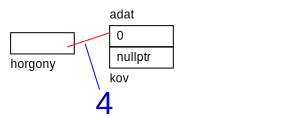
\includegraphics[width=\textwidth]{verem/verem05.pdf}
  \end{columns}
\end{frame}

%9
\begin{frame}
  \begin{columns}[c]
    \column{0.5\textwidth}
      \begin{exampleblock}{\textattachfile{verem2.cpp}{verem2.cpp}}
        \vspace{-.2cm}
        \small
        \lstinputlisting[style=cpp,linerange={4-16},numbers=left,firstnumber=4]{verem2.cpp}
        \vspace{-.2cm}
      \end{exampleblock}
    \column{0.45\textwidth}
      \includegraphics[width=\textwidth]{verem/verem06.pdf}
  \end{columns}
\end{frame}

%10
\begin{frame}
  \begin{columns}[c]
    \column{0.5\textwidth}
      \begin{exampleblock}{\textattachfile{verem2.cpp}{verem2.cpp}}
        \vspace{-.2cm}
        \small
        \lstinputlisting[style=cpp,linerange={4-16},numbers=left,firstnumber=4]{verem2.cpp}
        \vspace{-.2cm}
      \end{exampleblock}
    \column{0.45\textwidth}
      \includegraphics[width=\textwidth]{verem/verem07.pdf}
  \end{columns}
\end{frame}

%11
\begin{frame}
  \begin{columns}[c]
    \column{0.5\textwidth}
      \begin{exampleblock}{\textattachfile{verem2.cpp}{verem2.cpp}}
        \vspace{-.2cm}
        \small
        \lstinputlisting[style=cpp,linerange={4-16},numbers=left,firstnumber=4]{verem2.cpp}
        \vspace{-.2cm}
      \end{exampleblock}
    \column{0.45\textwidth}
      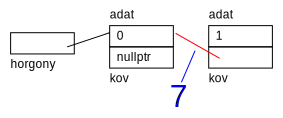
\includegraphics[width=\textwidth]{verem/verem08.pdf}
  \end{columns}
\end{frame}

%12
\begin{frame}
  \begin{columns}[c]
    \column{0.5\textwidth}
      \begin{exampleblock}{\textattachfile{verem2.cpp}{verem2.cpp}}
        \vspace{-.2cm}
        \small
        \lstinputlisting[style=cpp,linerange={4-16},numbers=left,firstnumber=4]{verem2.cpp}
        \vspace{-.2cm}
      \end{exampleblock}
    \column{0.45\textwidth}
      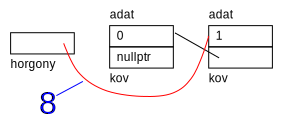
\includegraphics[width=\textwidth]{verem/verem09.pdf}
  \end{columns}
\end{frame}
